Instantaneous velocity is one of the simplest concepts in physics, but it is rather odd when you think about it more deeply. How can something be moving at a given moment? If it is stuck in a moment, how can it have any velocity? Isn't the instantaneous velocity at any moment in time just 0 as an object can't be in two places at one time? These are all philosophical questions I had when starting physics that were not quite addressed but that I came just to ignore. It is of little help to philosophize in these ways and, unfortunately, these lines of reasoning will not help us find anything useful. Even though philosophizing about physics is quite interesting, it is not particularly relevant for doing physics. Like Feynman and others have said, at many levels, we only understand the world at the level of the equations. The simple truth is that things can have a velocity at a given moment, and the velocity can be changing over time, but at any given moment it is fixed.

\
\vspace{5mm}
\\
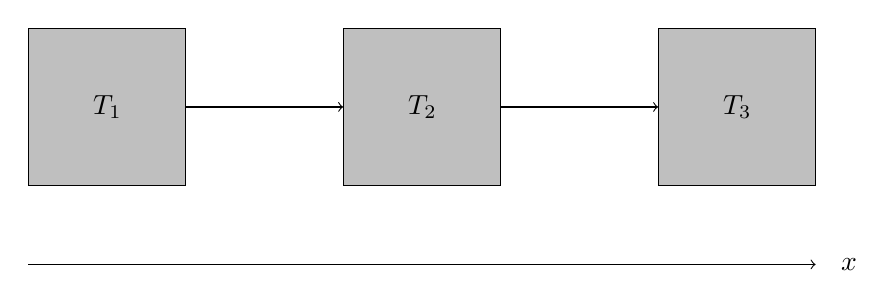
\begin{tikzpicture}
\filldraw[color = black, fill = lightgray] (0,0) rectangle (2,2);
\draw[black] (0.7,1) node[anchor=west] {$T_1$};
\draw[->] (2,1) -- (4,1);
\filldraw[color = black, fill = lightgray] (4,0) rectangle (6,2);
\draw[black] (4.7,1) node[anchor=west] {$T_2$};
\draw[->] (6,1) -- (8,1);
\filldraw[color = black, fill = lightgray] (8,0) rectangle (10,2);
\draw[black] (8.7,1) node[anchor=west] {$T_3$};
\draw[->] (0,-1) -- (10,-1);
\draw[black] (10.2,-1) node[anchor=west] {$x$};
\end{tikzpicture}

Defining the position as $x$ and assuming the motion is only in one definition, we can define the instantaneous velocity as
\begin{equation} \label{eq:a}
v\left(t\right) = \frac{dx}{dt}\end{equation}
at the moment $t$. With this definition, we are going to think of instantaneous velocity as the limit of the average velocity as the interval over which we are averaging goes to zero.  However, even though instantaneous velocity is defined in the way it is, I like to think about it a different way. $$v\left(t\right) = f\left(t\right)$$ for some velocity function $f\left(t\right)$. When we represent velocity in this way, we are thinking about velocity as a function of the force that is being imparted onto an object(which subsequently relies on time, thus we write $\left(t\right)$. We instead can think about instantaneous velocity as the velocity a particle would stay at if all forces acting on an object were suddenly removed at a given time. So when we have a constant force such as gravity imparting a force on an object, the instantaneous velocity will be the velocity of the object if that force were taken away. This may seem rather odd, but it can help elucidate some of our ideas of velocity and connect them to Newtonian dynamics which we will study soon. This is useful because velocity is fundamentally linked to the different forces on an object as we will see with Newton's laws. 

